To evaluate our system, we perform quantitative experiments on camera pose estimation accuracy, and qualitatively analyse the obtained reconstructions.
%To evaluate the performance of our system we perform experiments that draw comparisons in terms of quantitative pose estimation and qualitative reconstruction quality and efficacy.
Firstly, the pose estimation accuracy is evaluated via a well-established SLAM evaluation benchmark~\cite{sturm12iros}.
We like to point out that % with the primary difference being that with
in traditional dense SLAM systems~\cite{Prisacariu2014,Niessner2013,Newcombe2011} -- for which the benchmark is often employed -- the entire contents of the visible scene are used for pose estimation, whereas in our system we rely only on points belonging to the object's surface.
Whilst more challenging, this implicitly allows us to track the camera w.r.t. the object regardless of which of the two is subject to motion.
Then, qualitative comparisons are drawn between the reconstructions attained by our system, and those of the method described in \cite{Ren2013}.
We evaluate our system on multiple frame sequences depicting objects of different sizes. %; some with the object moving wrt. a fixed camera, others with the sensor in motion.% in the case of qualitative evaluation.

%\vspace{-.7\baselineskip}

\subsection{Pose Estimation Quality}
In this section we present quantitative results of our systems' %ability to maintain tracking
robustness in estimating the camera motion, by performing tracking against the reconstruction of a single object, instead of the whole scene.
The trajectories estimated by our system demonstrate low tracking drift. % and a robustness to loop closure events.
We perform such evaluation on two sequences of the RGB-D SLAM Dataset~\cite{sturm12iros} depicting static objects observed by a moving camera.
Tracking is performed using purely geometric clues, by matching the current depth frame with a rendering of the reconstructed object using a projective ICP tracking approach~\cite{Kahler2016}. We compare results against the system of \cite{Prisacariu2014} with object segmentation.
%, as such the evaluation is of camera pose estimation when tracking an object.
%By tracking the sensor pose against a subset of the observed scene 
%At this point it should be highlighted that our system is at a disadvantage when compared to dense SLAM systems that utilise the entire scene geometry for pose optimisation.

%In the following experiments, tracking is performed using only geometry cues from the rendered object models and the instantaneous depth frame.\\

The tracking accuracy is evaluated via the Absolute Trajectory Error (ATE) metric, as outlined in \cite{sturm12iros}, and is summarised in Table~\ref{ateTable}.

\begin{table}[!t]
	{
        \footnotesize
		\begin{center}
			\begin{tabular}{l@{\hskip 1cm} c c}
				\emph{Sequence Name} & \emph{Our Approach ATE (m)} & \emph{InfiniTAM ATE (m)}\\
				\midrule
				\textsf{freiburg3\_cabinet} & 0.077903 & 0.520693\\
				\textsf{freiburg3\_teddy}   & 0.030596 & 0.048560 
			\end{tabular}
		\end{center}
	}
	\caption{ATE(Absolute Trajectory Error) results (lower is better) achieved by our approach versus InfinITAM with object segmentation.}
	\label{ateTable}
\end{table}

\begin{figure}[!t]
	\centering
	\begin{tabular}{cc}
		%\fbox{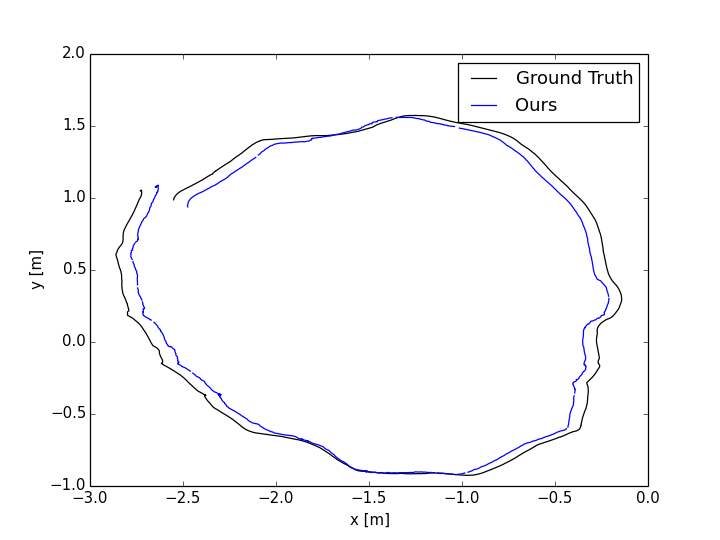
\includegraphics[width=0.2\textwidth]{results/rgbd_dataset_freiburg3_cabinet.png}} & %\fbox{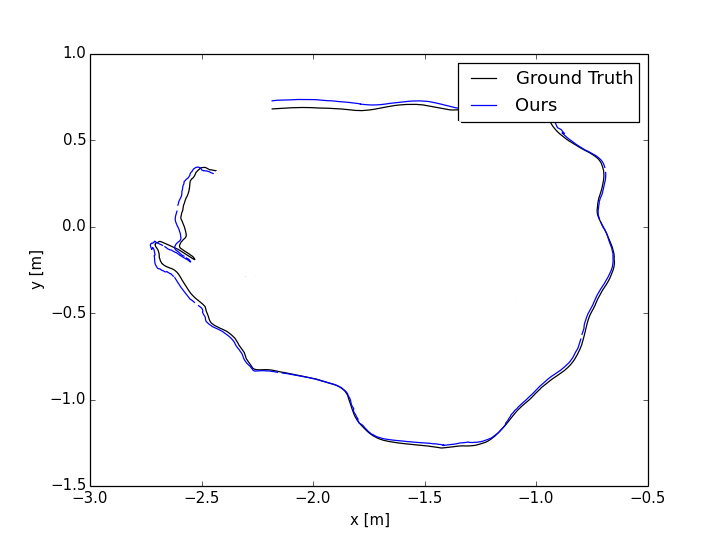
\includegraphics[width=0.2\textwidth]{results/rgbd_dataset_freiburg3_teddy.png}}
		\fbox{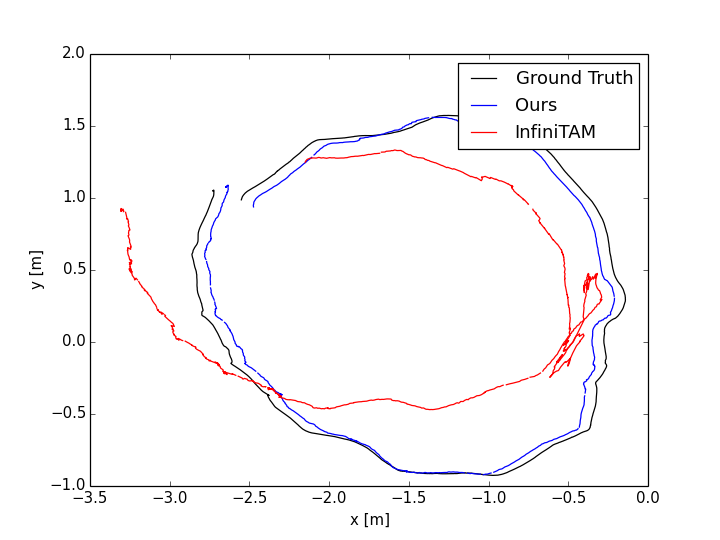
\includegraphics[width=0.2\textwidth]{results/comparative_cabinet.png}} &
		\fbox{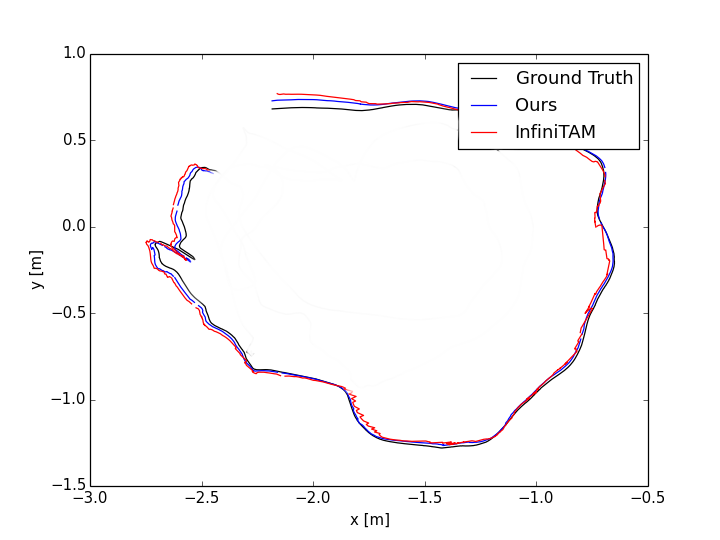
\includegraphics[width=0.2\textwidth]{results/comparative_teddy_clean.png}}
	\end{tabular}
	\caption{
        Comparison of the estimated camera trajectory with the ground truth for
		\textbf{(L)}~\textit{freiburg3\_cabinet}  and
		\textbf{(R)}~\textit{freiburg3\_teddy}.
	}
\label{fig:tumTrajectories}
\end{figure}

At this point, it should be highlighted that our proposed system is at a disadvantage when compared to dense SLAM systems that utilise the entire scene geometry for pose optimisation, since we track the sensor pose against a subset of the observed scene.
Nevertheless, as shown by the results in Figure~\ref{fig:tumTrajectories}, our system is able to robustly estimate trajectories close to the ground truth whilst using only the objects' geometric appearance.
Quantitatively, the tracking accuracy is evaluated via the Absolute Trajectory Error (ATE) metric, as outlined by \cite{sturm12iros}.
The cabinet reconstructed in the \textit{freiburg3\_cabinet} sequence is lacking in geometric features, as the object is mostly planar,
%It can be seen that there is a
and the small deficit in tracking quality is mostly due to this factor.
However, our system remains able to estimate a fairly accurate trajectory. 
In the \textit{freiburg3\_teddy} sequence we determine a trajectory very close to the ground truth.
Improvement over the accuracy in \textit{freiburg3\_cabinet} is due to the wider availability of geometrical features, such as curves in the teddy's body and head.

\subsection{Qualitative Reconstruction Quality}
In this section we present a qualitative comparison of our method vs. the approach by Ren et~al.~\cite{Ren2013} in the reconstruction of closed object models. %by relying on a variety of sequences and demonstrating efficacy over \cite{Ren2013} in this regard.
Each sequence is run through both systems; to evaluate the obtained results we regularly take snapshots of the reconstruction, in the case of our system, and the level set evolutions, in the case of Ren et al.
Such snapshots are captured after each quarter of a sequence has been processed. %quarterly intervals of the systems run time through the sequence.

\begin{figure}[!t]
	\centering
	\begin{tabular}{cc}
		\fbox{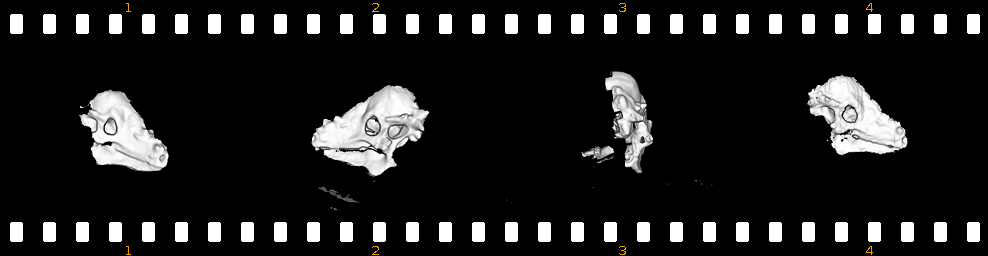
\includegraphics[width=0.45\textwidth]{filmstrips/dino.png}} \\ [2ex]
		\fbox{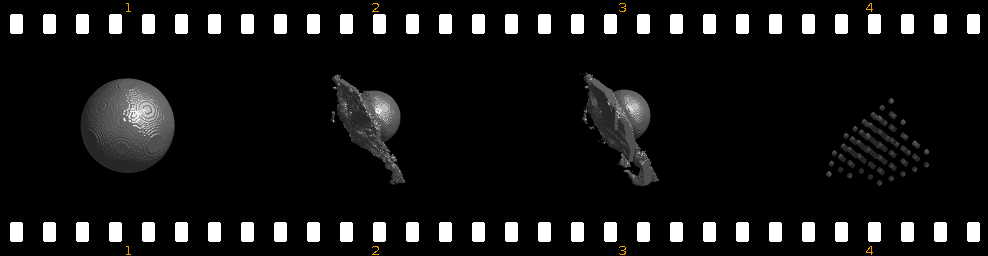
\includegraphics[width=0.45\textwidth]{filmstrips/dino_s3d_large.png}}
	\end{tabular}
	\caption{
        Quarterly interval snapshots of the Dinosaur Head reconstruction using \textbf{(Upper)} our method, and \textbf{(Lower)} the one proposed by Ren et~al.~\cite{Ren2013}.
	}
	\label{fig:dinoComparison}
\end{figure}

\begin{figure*}[!t]
	\centering
	\begin{tabular}{cccc}
		\fbox{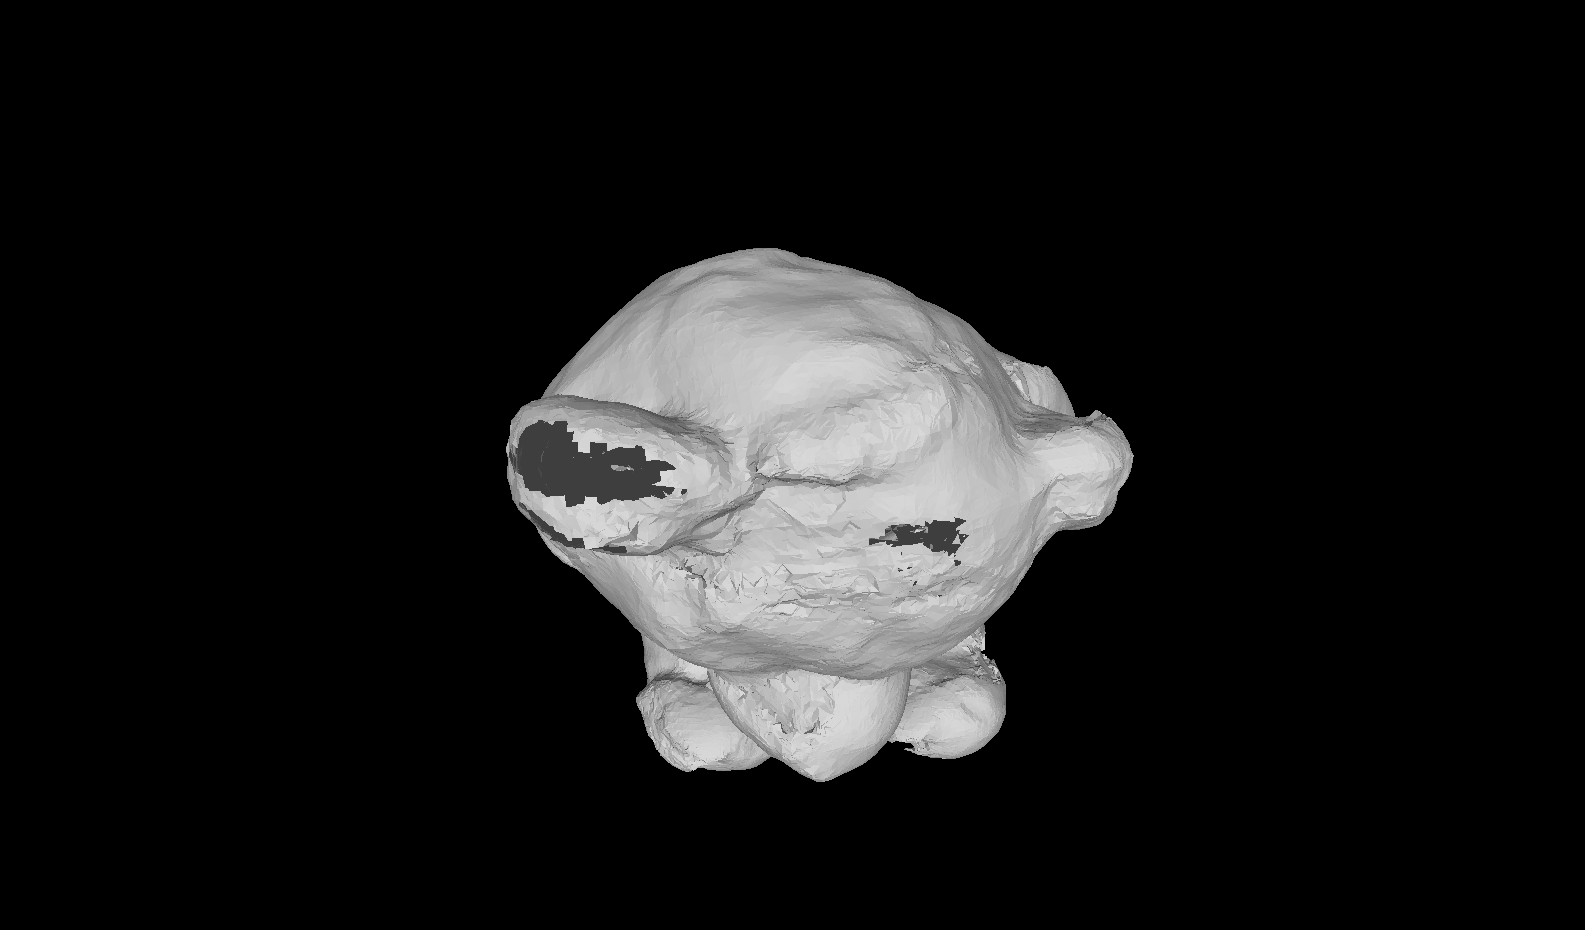
\includegraphics[width=3cm]{screenshots/untextured/teddy_top00.png}}&
		\fbox{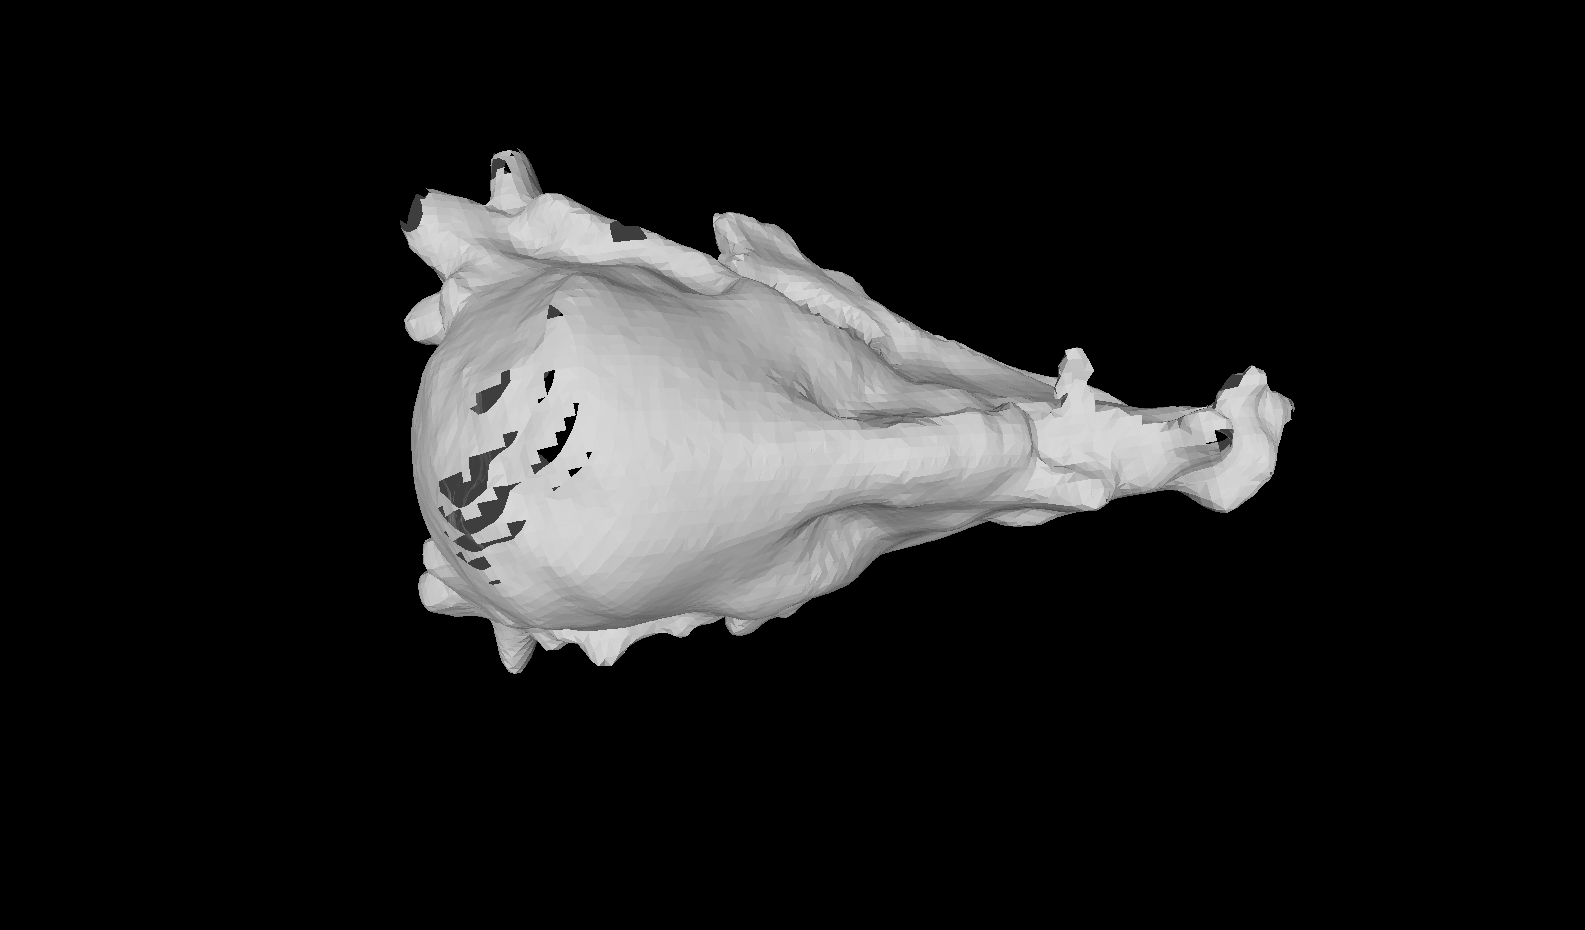
\includegraphics[width=3cm]{screenshots/untextured/dino_top00.png}}&
		\fbox{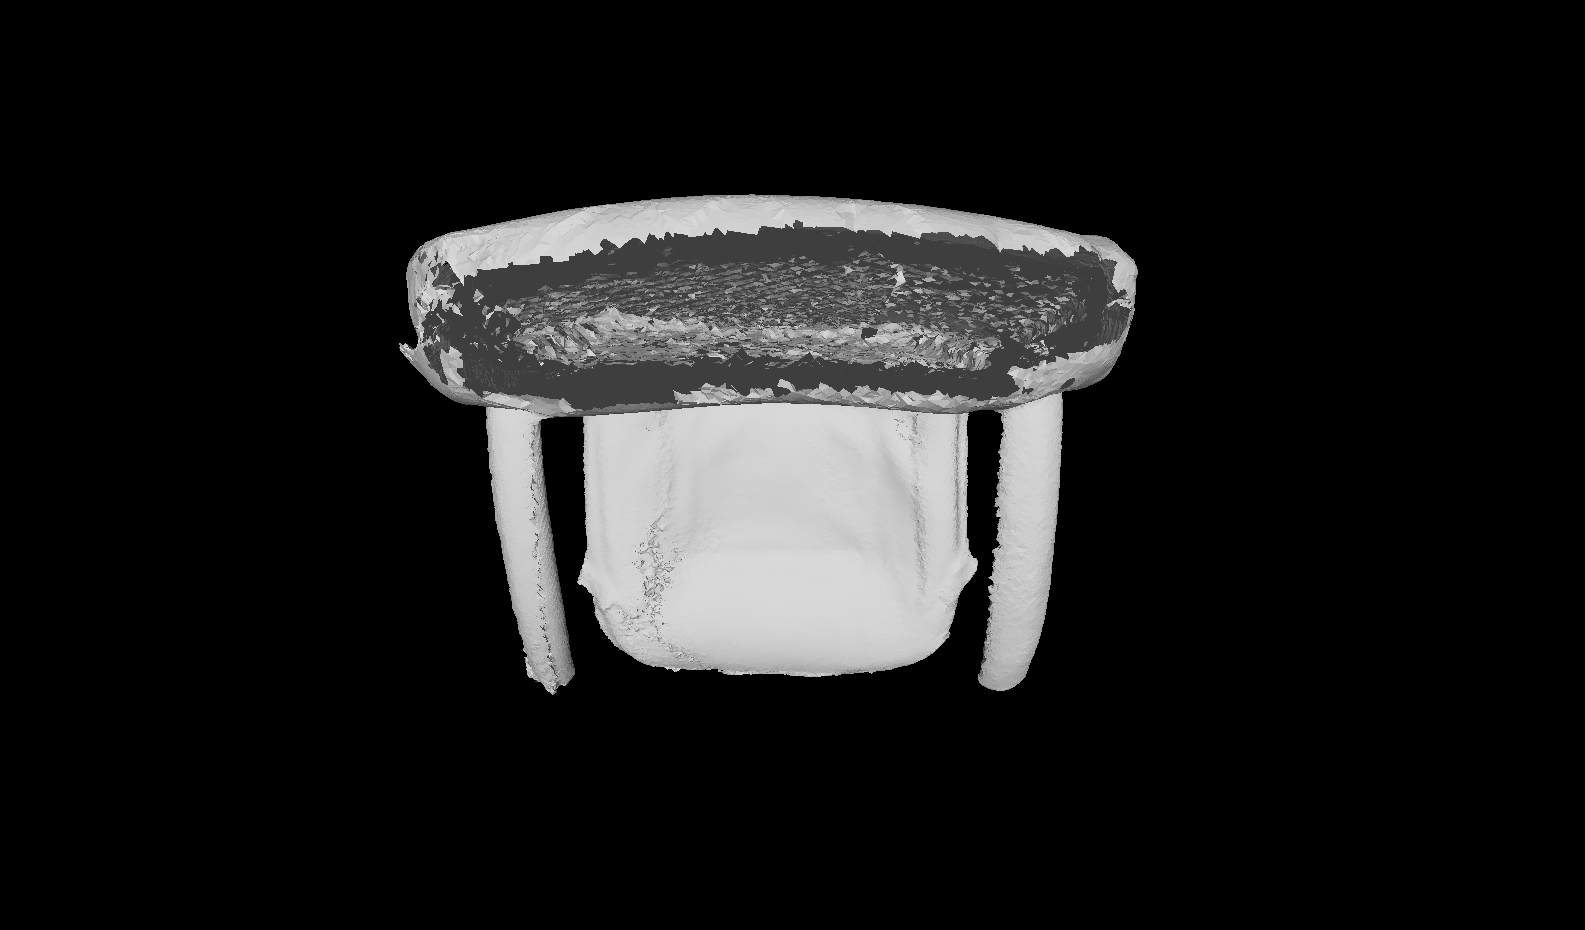
\includegraphics[width=3cm]{screenshots/untextured/chair_top00.png}}&
		\fbox{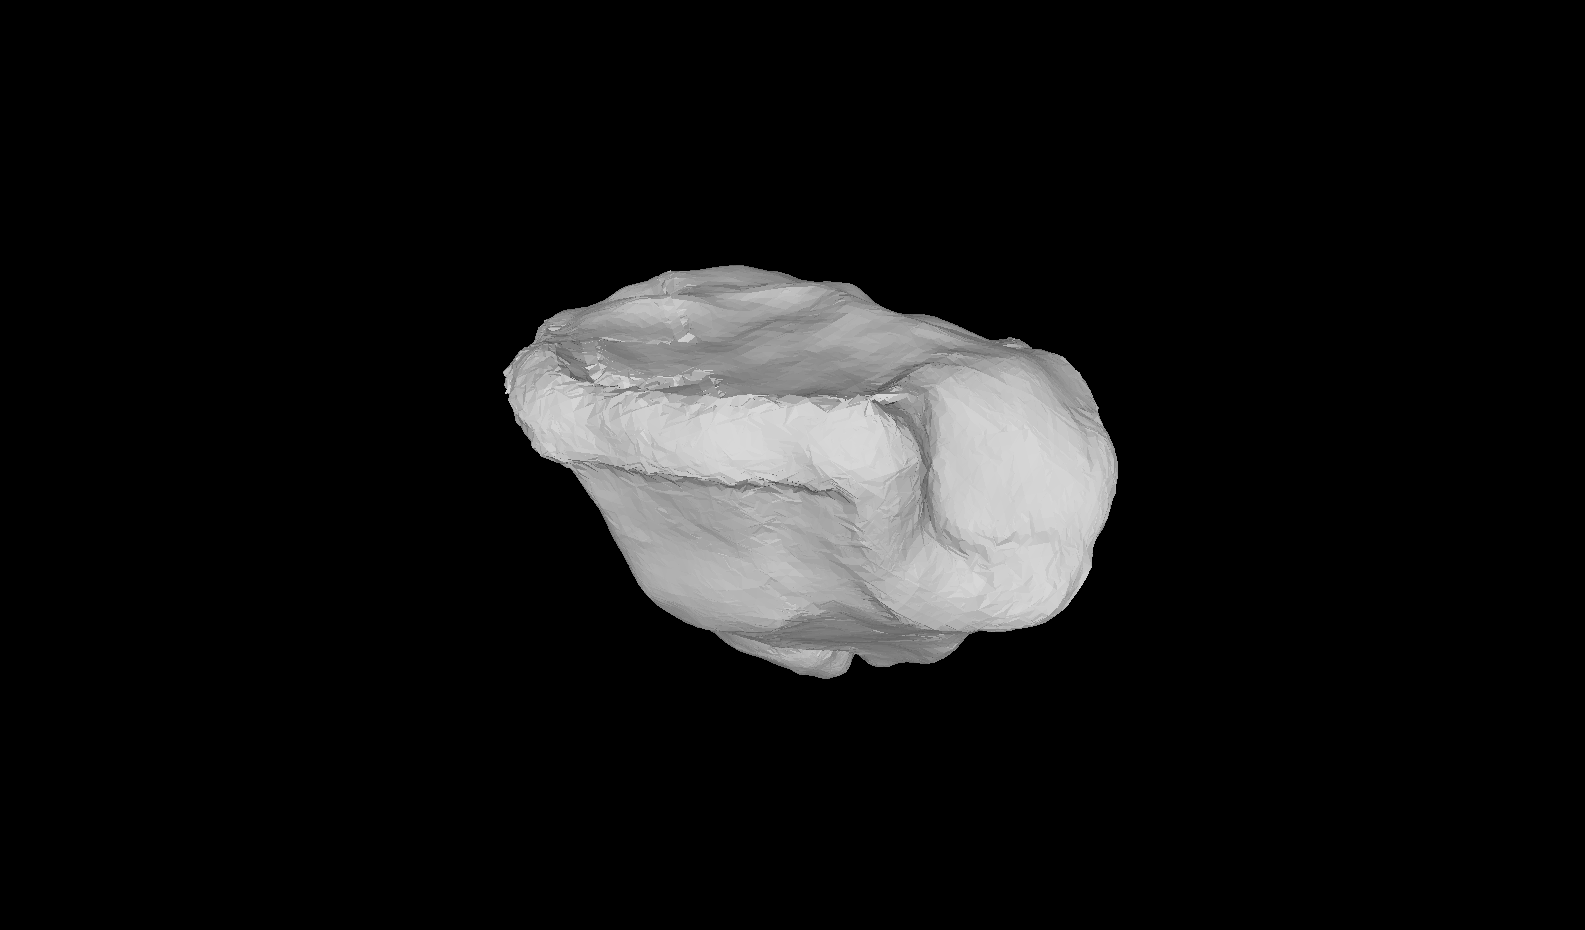
\includegraphics[width=3cm]{screenshots/untextured/rock_top00.png}}\\
		(a) & (b) & (c) & (d)
	\end{tabular}
	\caption{
		Closed reconstructions of (b) a Teddy, (b) a Dinosaur Head, (c) a Chair, and (d) a Rock.
	}
	\label{fig:top_shots}
%	\vspace{-\baselineskip}
\end{figure*}

\begin{figure}[!t]
	\centering
	\begin{tabular}{cc}
		\fbox{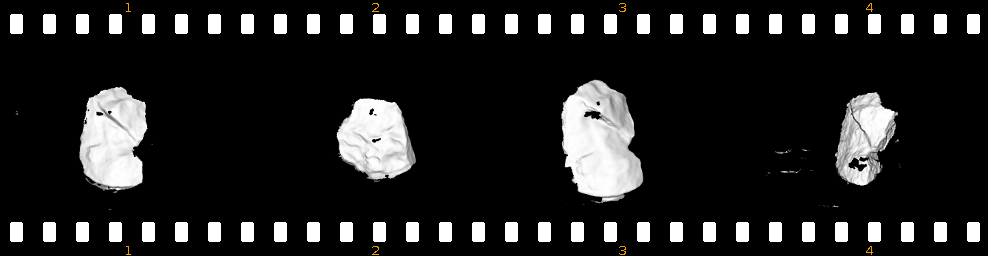
\includegraphics[width=0.45\textwidth]{filmstrips/rock.png}} \\ [2ex]
		\fbox{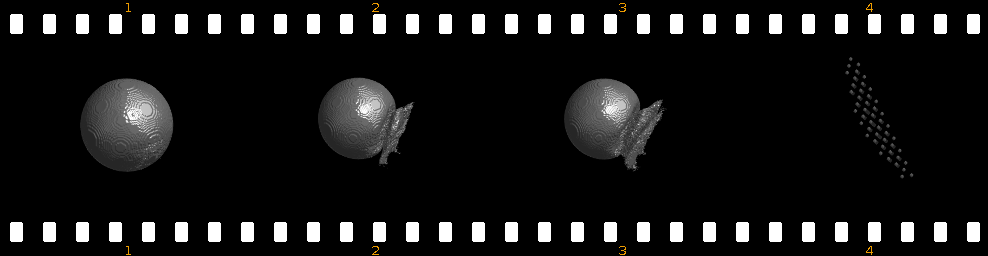
\includegraphics[width=0.45\textwidth]{filmstrips/rock_s3d_large.png}}
	\end{tabular}
	\caption{
		Quarterly interval snapshots of the Museum Rock reconstruction using \textbf{(Upper)} our method, and \textbf{(Lower)} the one proposed by Ren et~al.~\cite{Ren2013}.
	}
	\label{fig:rockComparison}
\end{figure}

As depicted in Figure~\ref{fig:dinoComparison}, our method is able to successfully reconstruct the Dinosaur Head, whereas the approach by Ren~et~al. fails to converge towards a feasible shape.
In addition, Figure~\ref{fig:top_shots} demonstrates that our system is able to generate consistent models (unaffected by camera tracking drift) for a variety of sequences containing several loop closures.
Failure of the competing method %of Ren et al
is also apparent for other sequences evaluated in this work, all presenting failure cases analogous to Figure~\ref{fig:dinoComparison}(R). % to converge to a correct shape.
%Such examples will be presented in the supplementary materials.
%The supplementary materials to this work demonstrate our efficacy vs that of Ren et al \cite{Ren2013}.\\
Another such example may be observed in Figure \ref{fig:rockComparison}.

The object reconstructions depicted in Figure~\ref{fig:demo} have been obtained from sequences in which a camera was moved in a loop around each object in order to generate a closed model.

In addition, we provide a qualitative comparison between the reconstructions produced by the KinectFusion implementation of \cite{Prisacariu2014} when 
tracking the entire scene and manually segmenting the object out as a post processing versus our online segmentation and reconstruction system. This 
comparison is visible in Figure \ref{}

\begin{figure*}[!t]
	\centering
	\begin{tabular}{cccc}
		\fbox{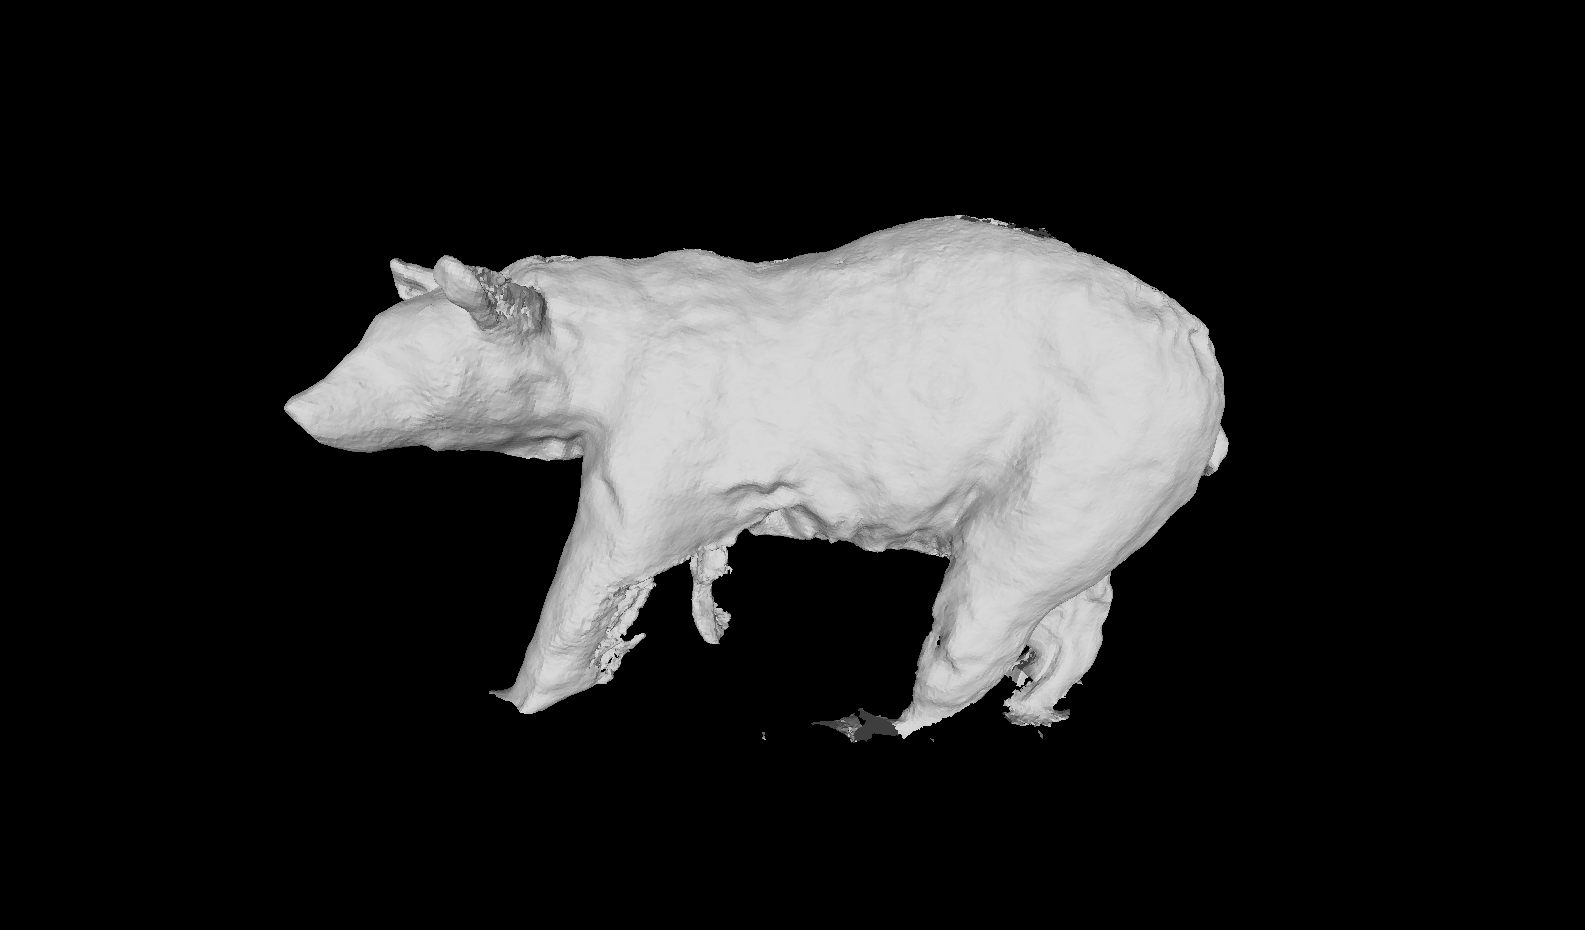
\includegraphics[width=3cm]{screenshots/Comparison Stills/InfiniTAM/bear00.png}}&
		\fbox{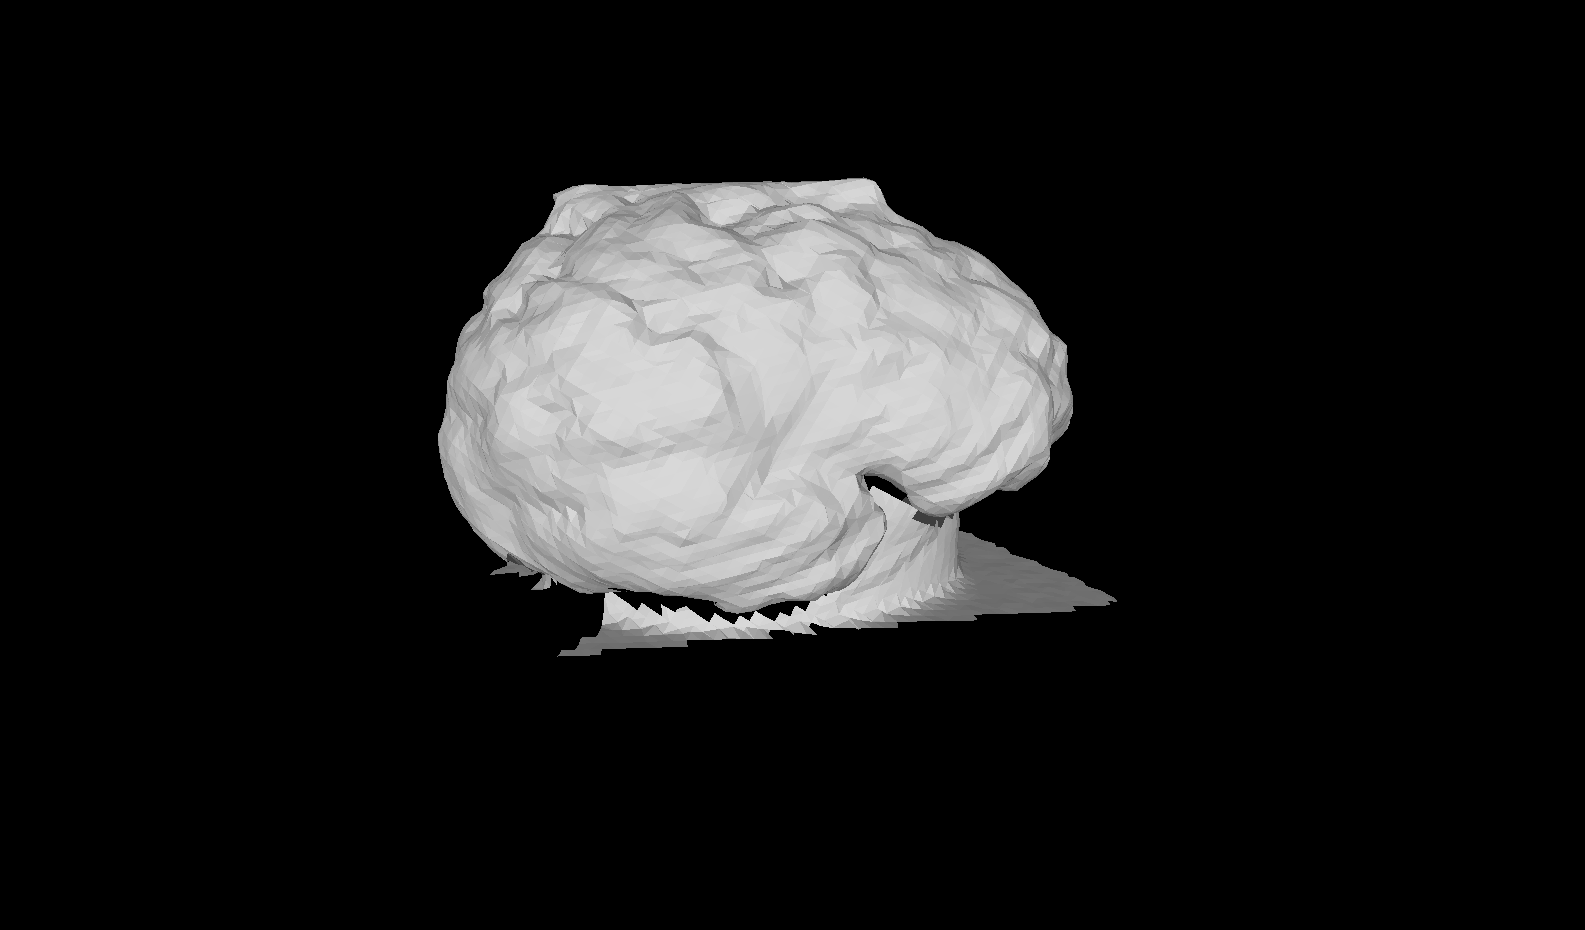
\includegraphics[width=3cm]{screenshots/Comparison Stills/InfiniTAM/brain00.png}}&
		\fbox{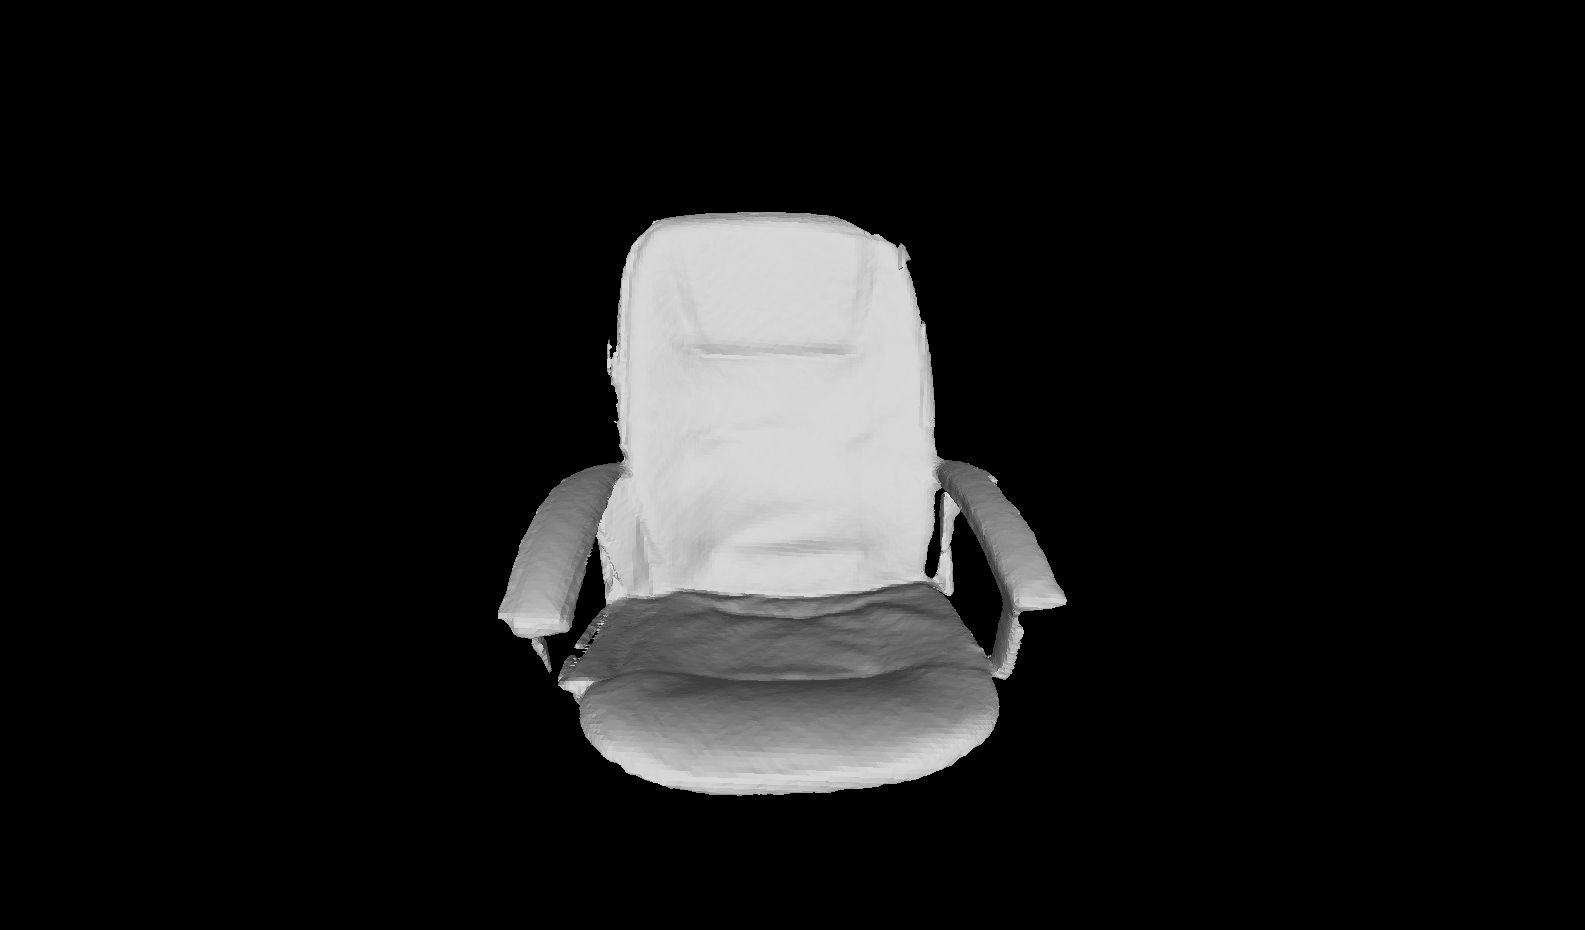
\includegraphics[width=3cm]{screenshots/Comparison Stills/InfiniTAM/chair00.png}}&
		\fbox{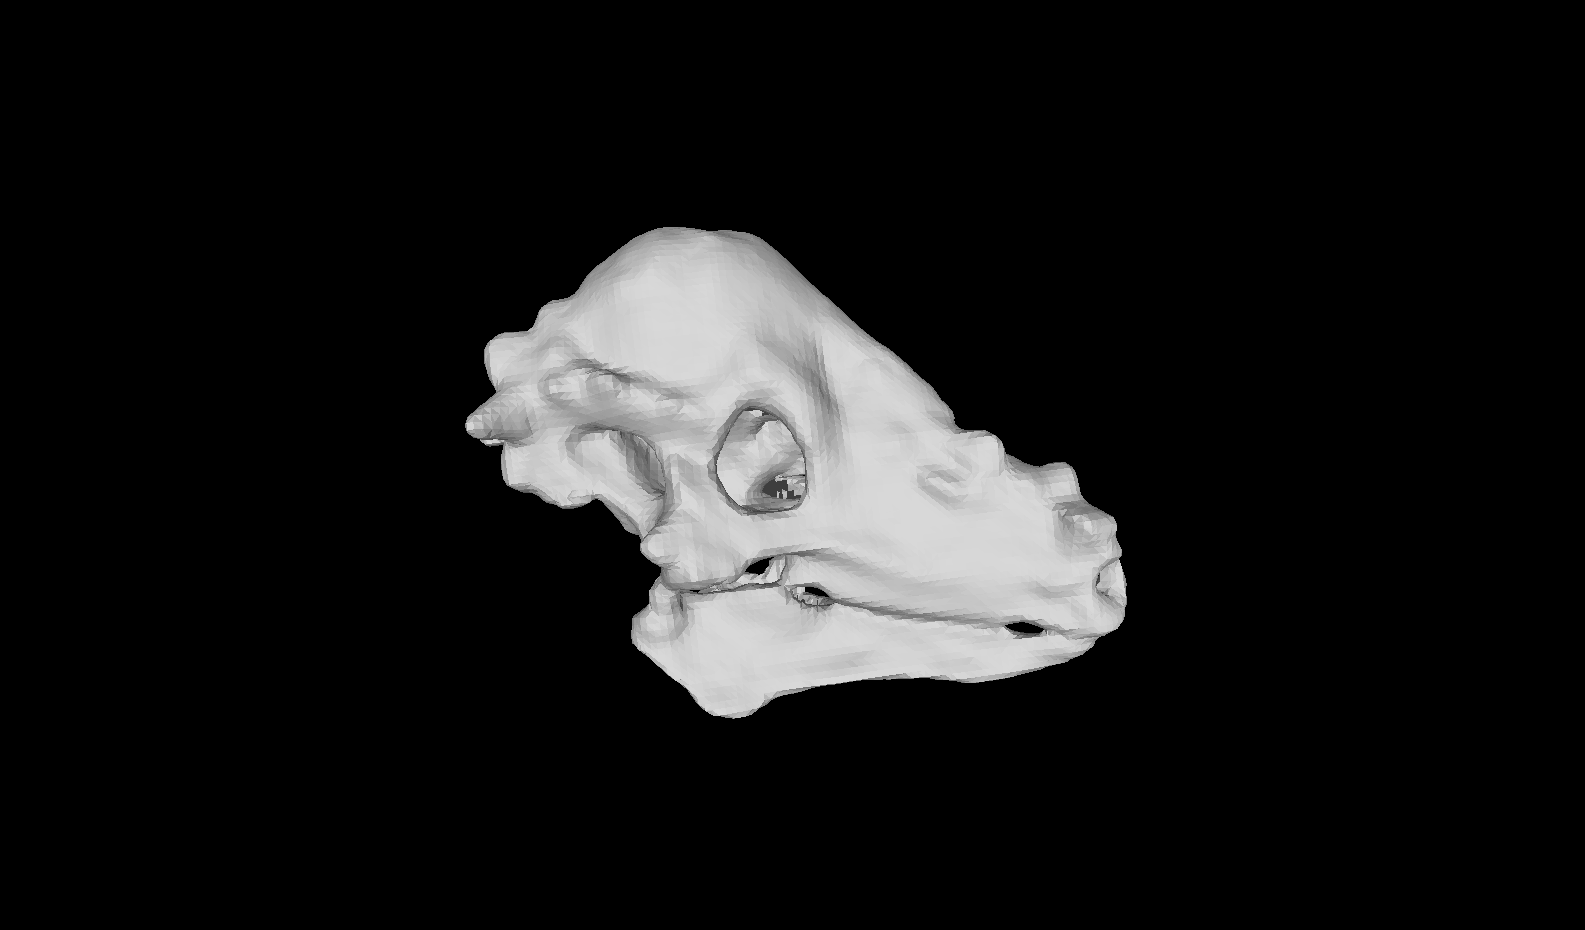
\includegraphics[width=3cm]{screenshots/Comparison Stills/InfiniTAM/dino00.png}}\\
		(a)&(b)&(c)&(d) \\ 
		\fbox{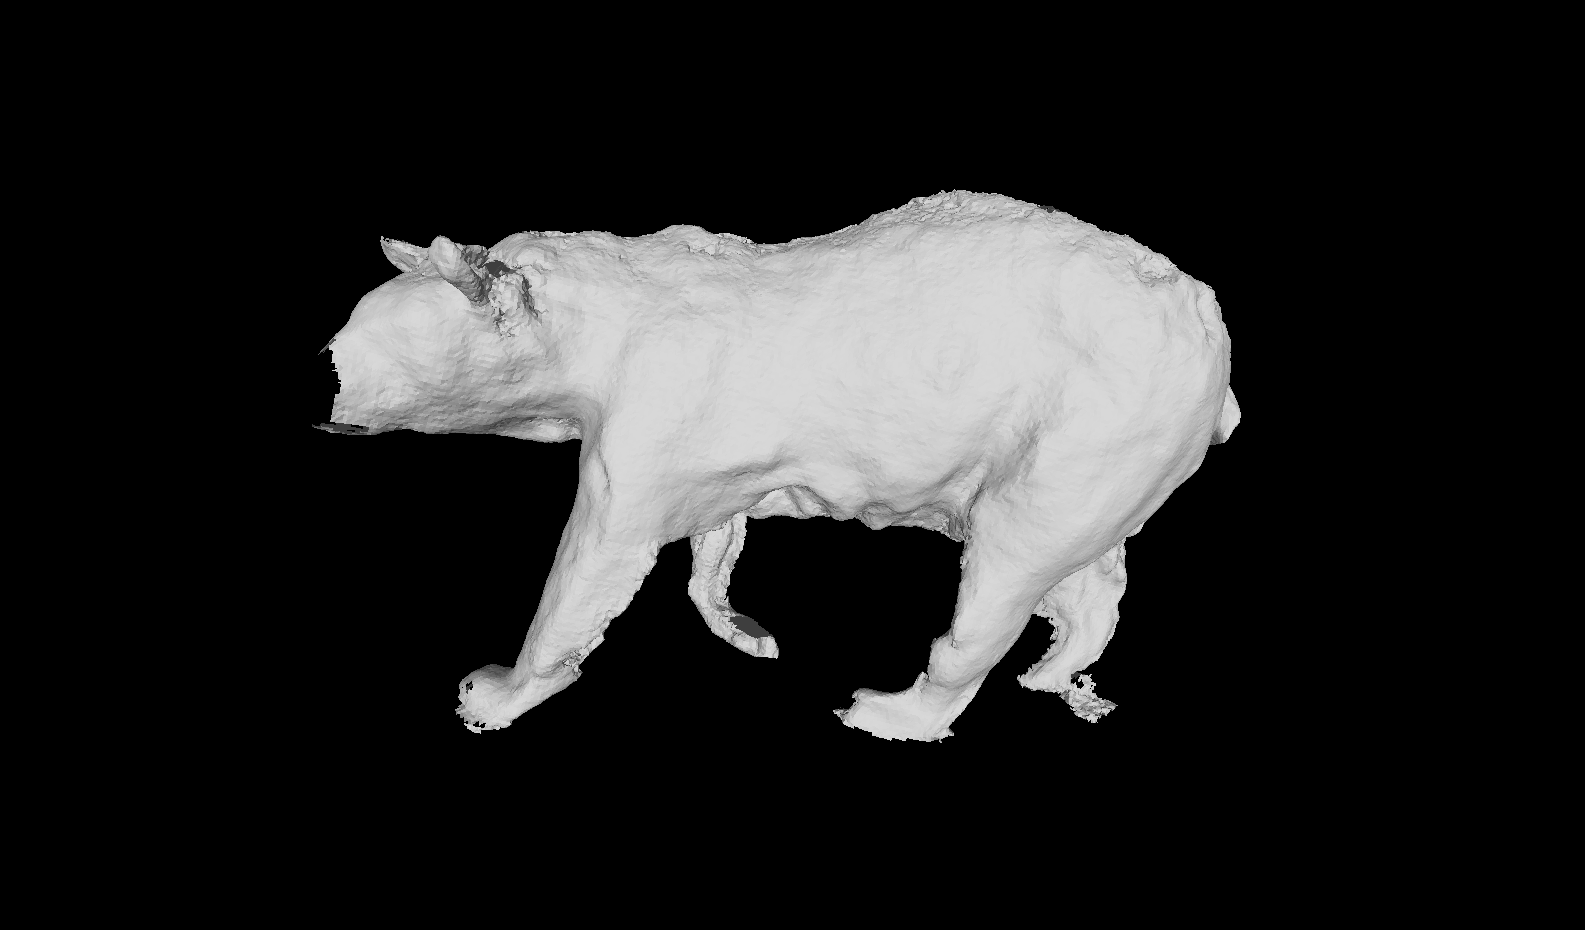
\includegraphics[width=3cm]{screenshots/Comparison Stills/ProbObjects/bear00.png}}&
		\fbox{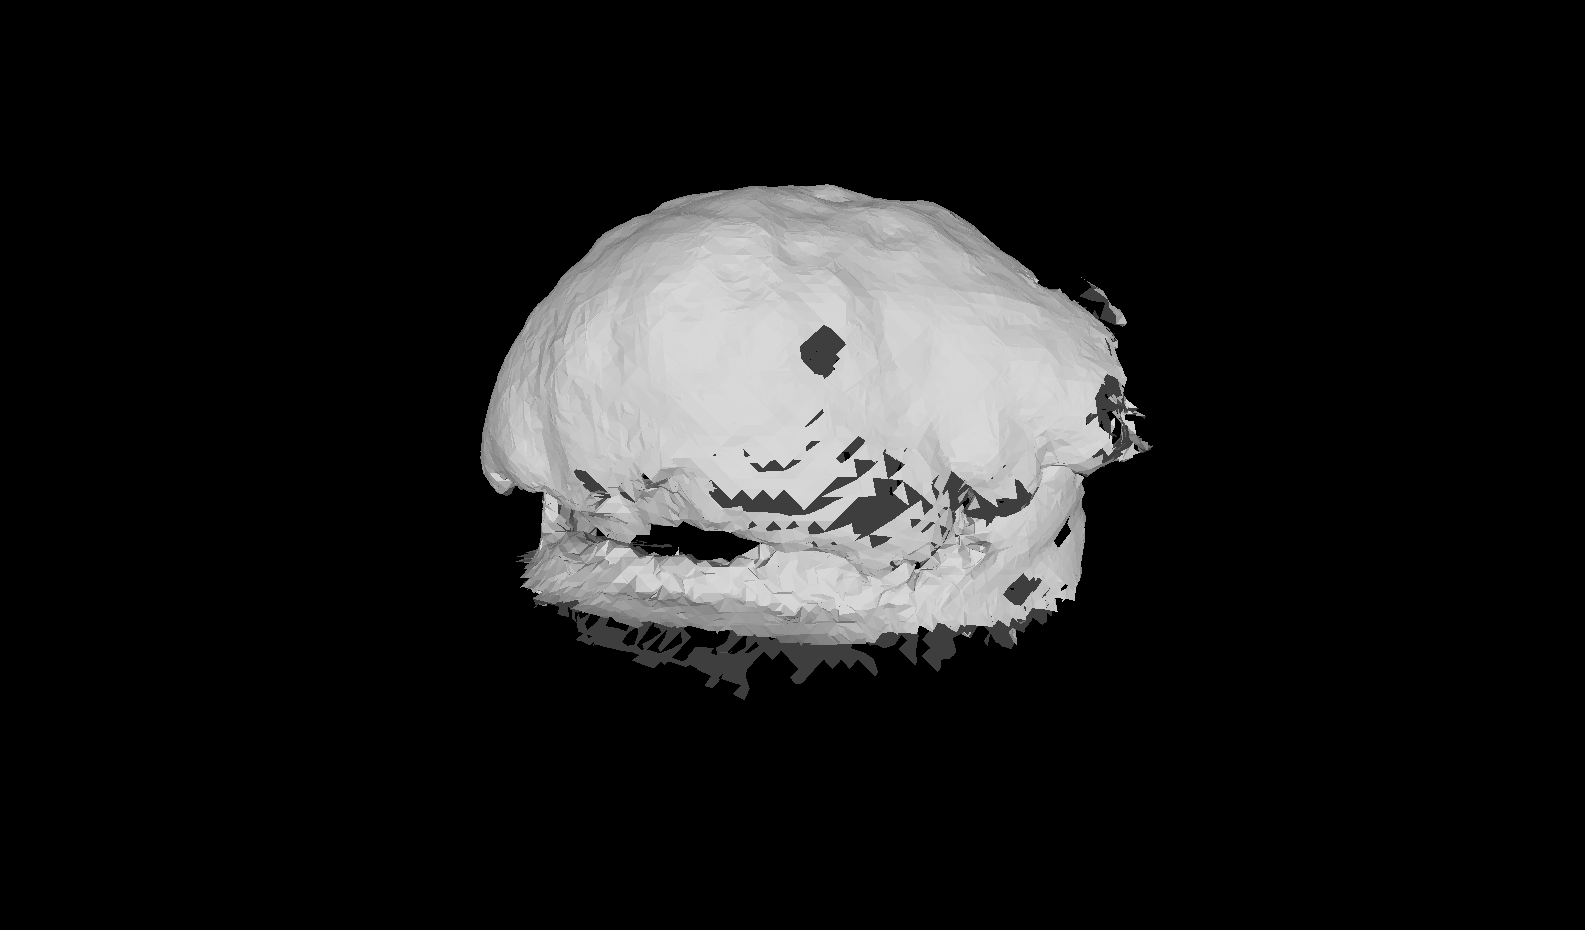
\includegraphics[width=3cm]{screenshots/Comparison Stills/ProbObjects/brain00.png}}&
		\fbox{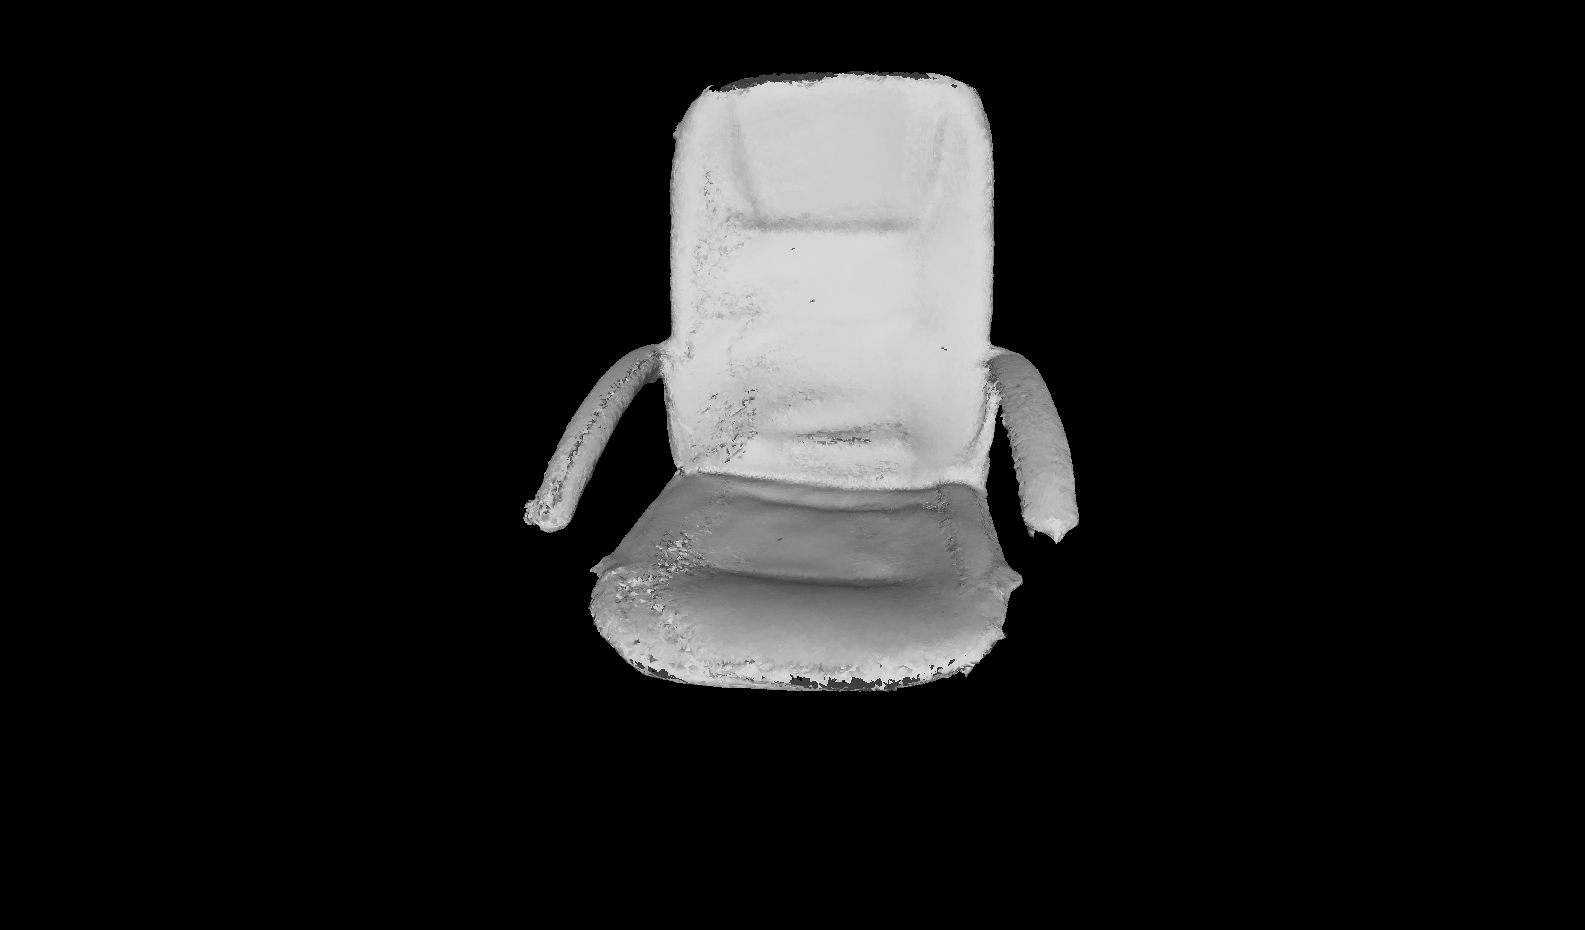
\includegraphics[width=3cm]{screenshots/Comparison Stills/ProbObjects/chair00.png}}&
		\fbox{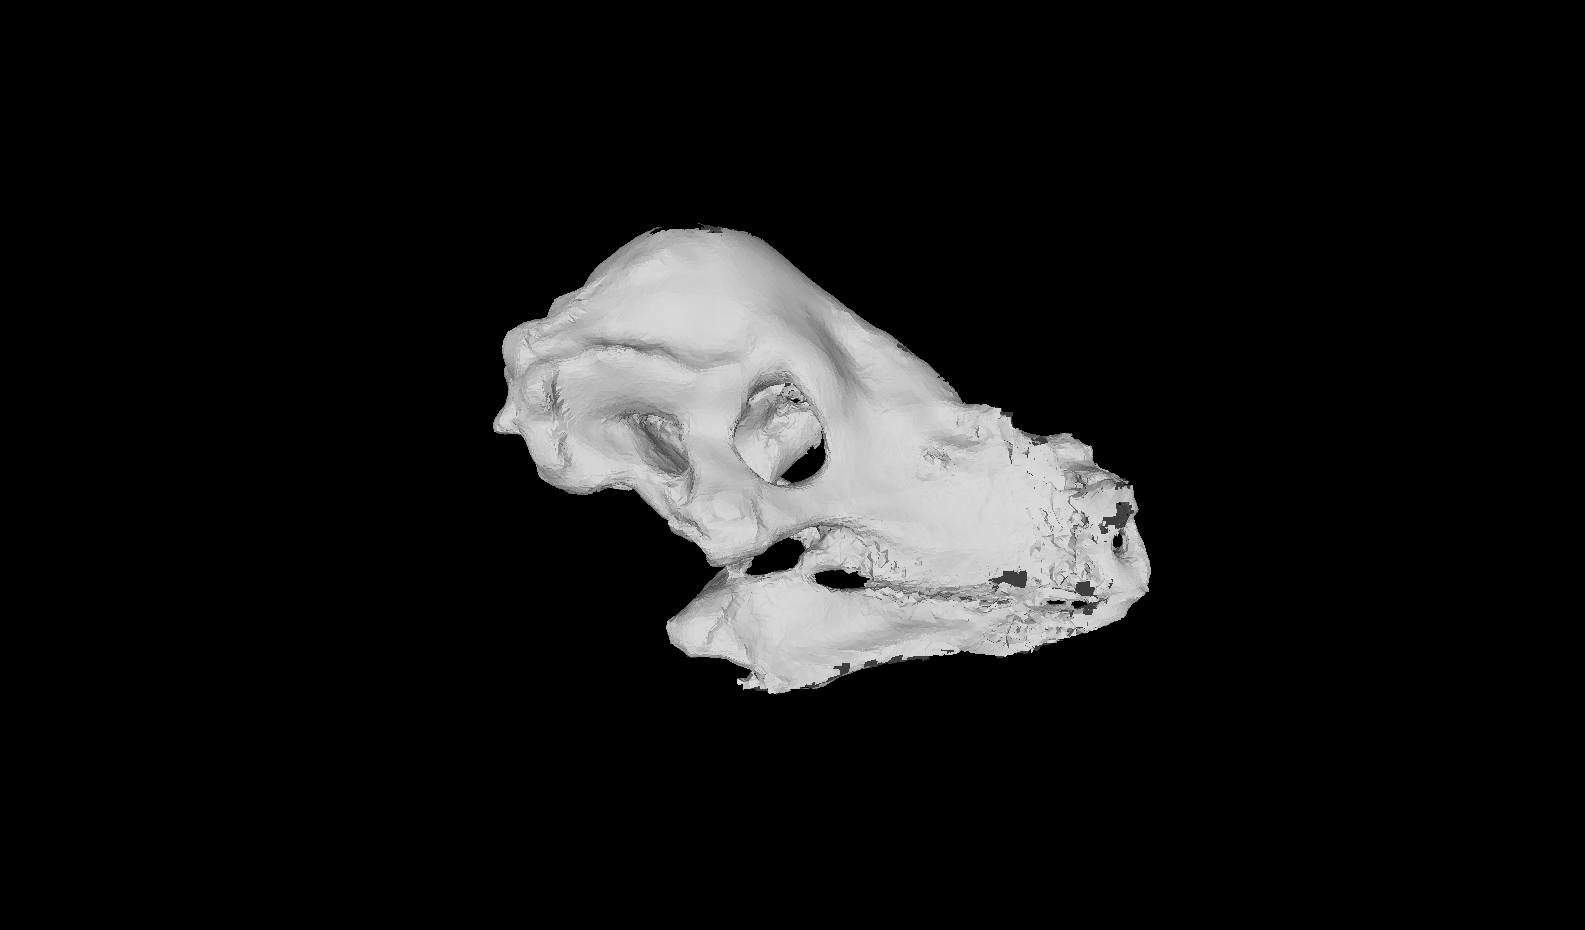
\includegraphics[width=3cm]{screenshots/Comparison Stills/ProbObjects/dino00.png}}\\
		(e)&(f)&(g)&(h) \\ 
	\end{tabular}
	\vspace{1mm}
	\caption{
		Reconstruction examples using InfiniTAM:
		\textbf{(a)} Bear,
		\textbf{(b)} Brain,
		\textbf{(c)} Chair,
		\textbf{(d)} Dino Head.
		Reconstruction examples using our system:
		\textbf{(e)} Bear,
		\textbf{(f)} Brain,
		\textbf{(g)} Chair,
		\textbf{(h)} Dino Head.
	}
	%	\vspace{-5mm}
	\label{fig:demo}
\end{figure*}

%As can be seen from the top down views of Figure \ref{fig:top_shots}, our system is capable of producing closed models, unaffected by tracking drift and loop closure events.

\subsection{Quantitative Reconstruction Quality}
In this section we perform a quantitative evaluation of reconstruction quality of our method against an established dense SLAM system \cite{Prisacariu2014} following the KinectFusion \cite{Newcombe2011} pipeline.
The outputted meshes of our model are compared with the meshes of the dense SLAM system with the object of interest manually segmented out from the remainder of the scene. To quantify the reconstruction quality 
we employ the Hausdorff Distance for subsets of metric spaces, where in our case the metric space is Euclidean. The Hausdorff Distance is defined as follows
\begin{equation}
\begin{split}
d_{H}(X, Y) = \max \Bigg \{ \sup_{x \in X} \inf_{y \in Y} d(x, y), \sup_{y \in Y} \inf_{x \in X} d(x, y) \Bigg \}
\end{split}
\end{equation}
where $X$ is the mesh for the ground truth dense SLAM reconstruction, $Y$ is the mesh outputted by our system and $d(.)$ is the Euclidean distance.

The resultant comparisons may be found in table \ref{hausdorffTable}. In addition, we provide the outputted reconstructions from our system textured on reconstruction quality w.r.t. the Hausdorff Distance. 
For reference, the colour scale used is given in figure \ref{fig:hausdorffTextured} where the left extrema(blue) is given by a sequences \textit{Max Dist} and the right extrema(red) by the sequences \textit{Min Dist}. 
\begin{table}[!t]
	{
		\footnotesize
		\begin{center}
			\begin{tabular}{l c c c c}
				\emph{Sequence} & \emph{Min Dist} & \emph{Max Dist} & \emph{Mean Dist} & \emph{RMS}\\
				\midrule
				\textsf{Bear} & 0 & 0.102777 & 0.013588 & 0.019796 \\
				\textsf{Brain} & 0 & 0.026465 & 0.008745 & 0.011349 \\
				\textsf{Chair} & 0 & 0.053441 & 0.012349 & 0.016422 \\
				\textsf{Dino} & 0 & 0.035252 & 0.007919 & 0.010676
			\end{tabular}
		\end{center}
	}
	\caption{Hausdorff Distance measurements between ground truth mesh and our systems output.}
	\label{hausdorffTable}
\end{table}

\begin{figure*}[!t]
	\centering
	\begin{tabular}{cccc}
		\fbox{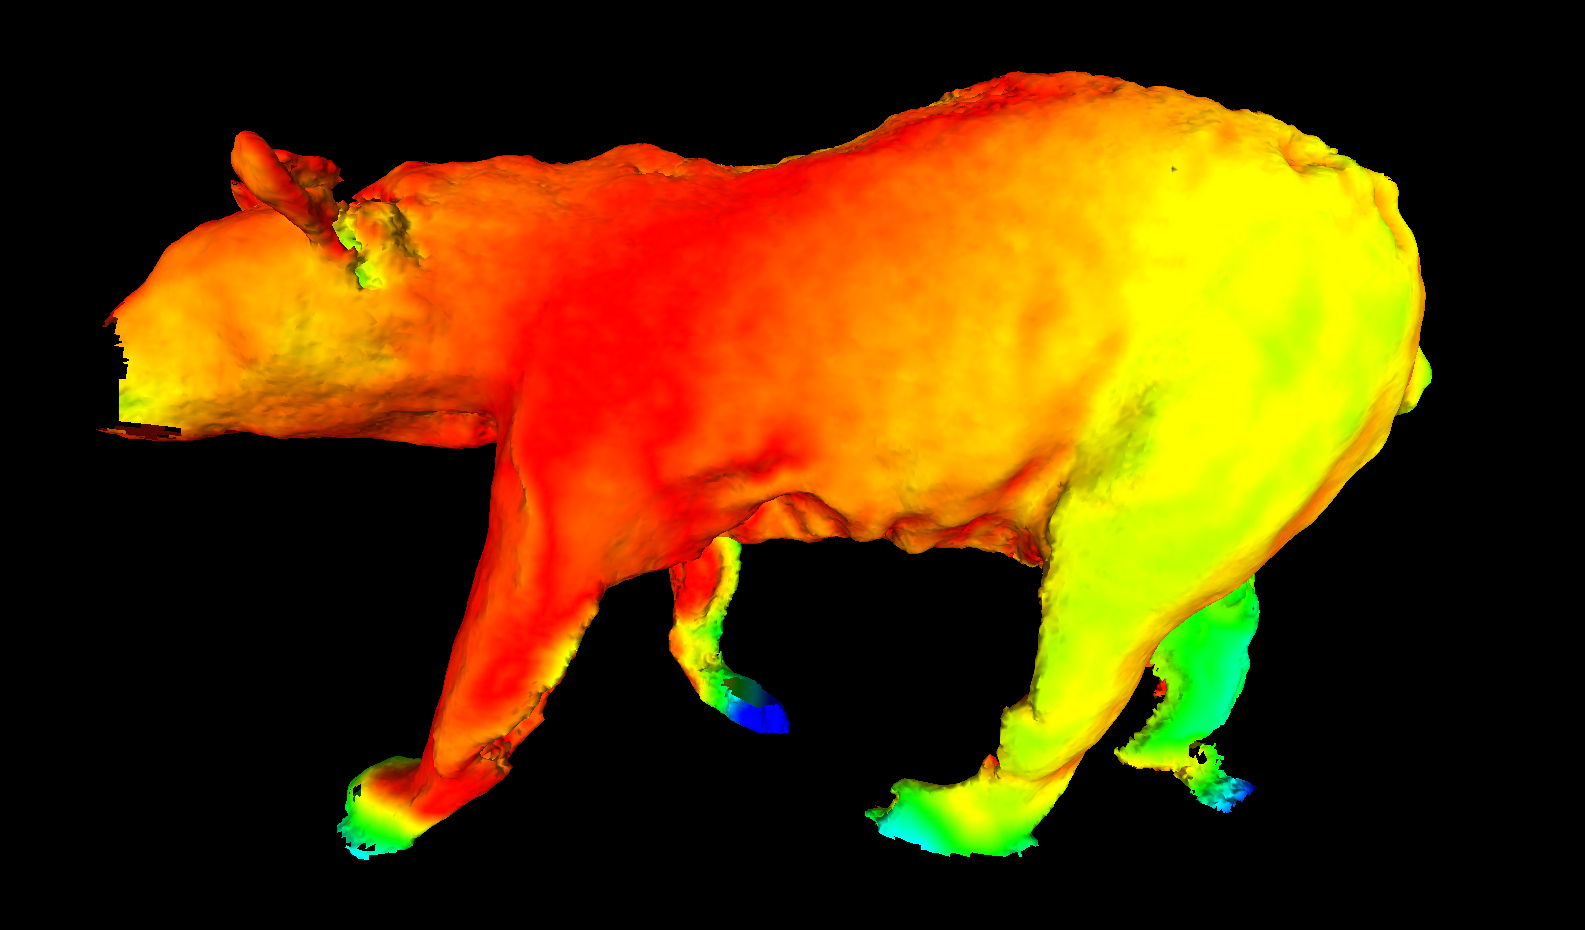
\includegraphics[width=3cm]{hausdorff/bear.png}}&
		\fbox{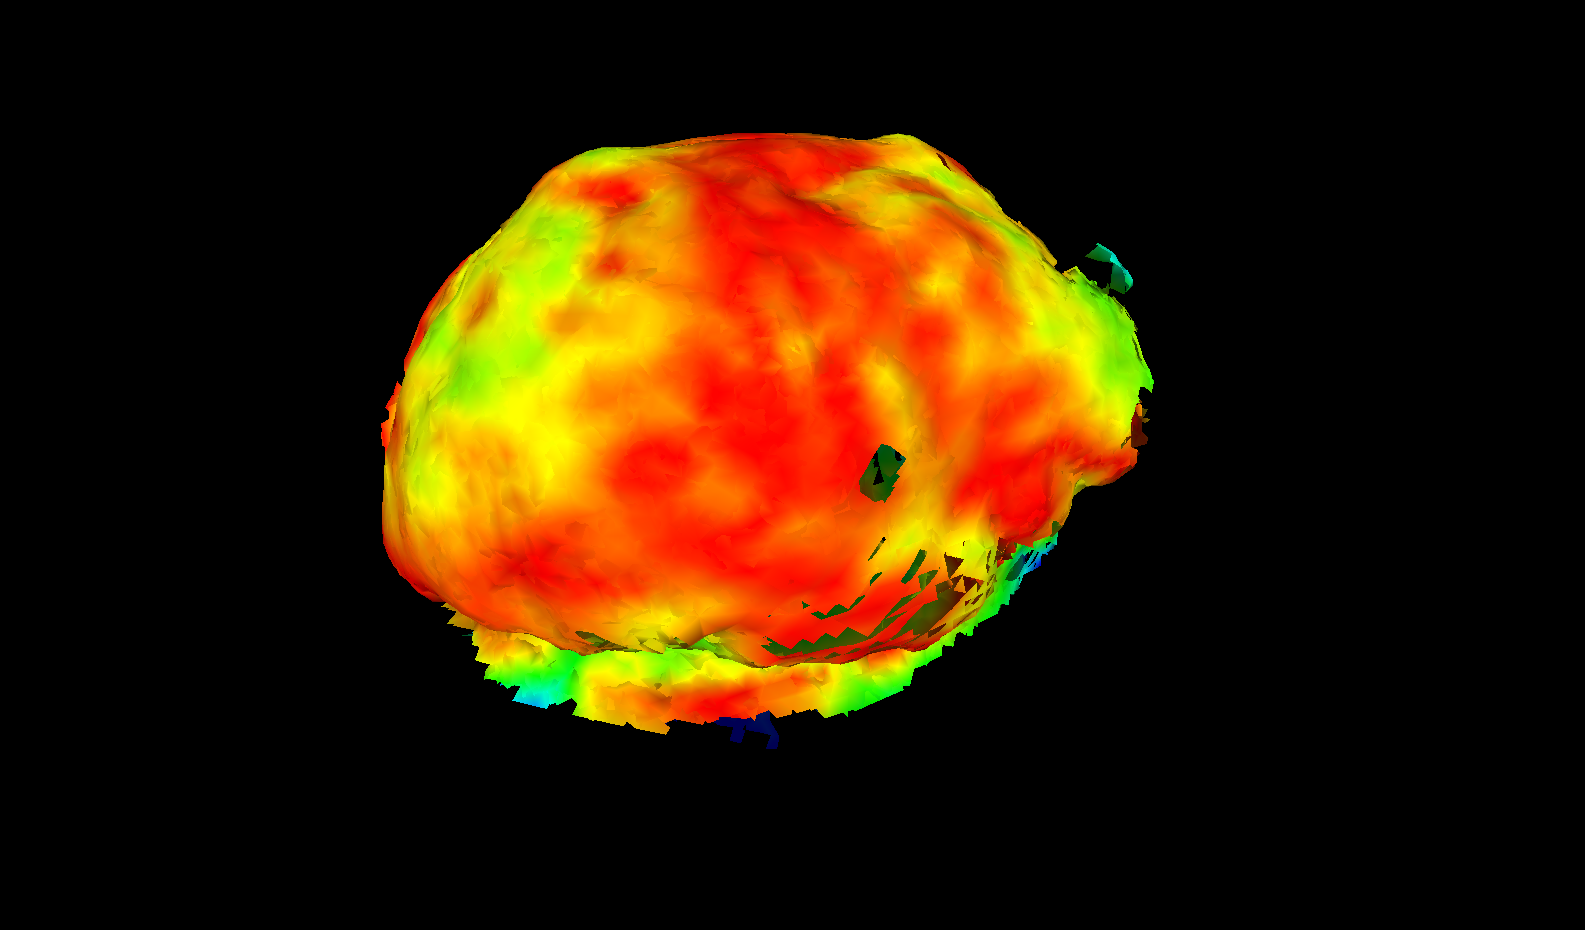
\includegraphics[width=3cm]{hausdorff/brain.png}}&
		\fbox{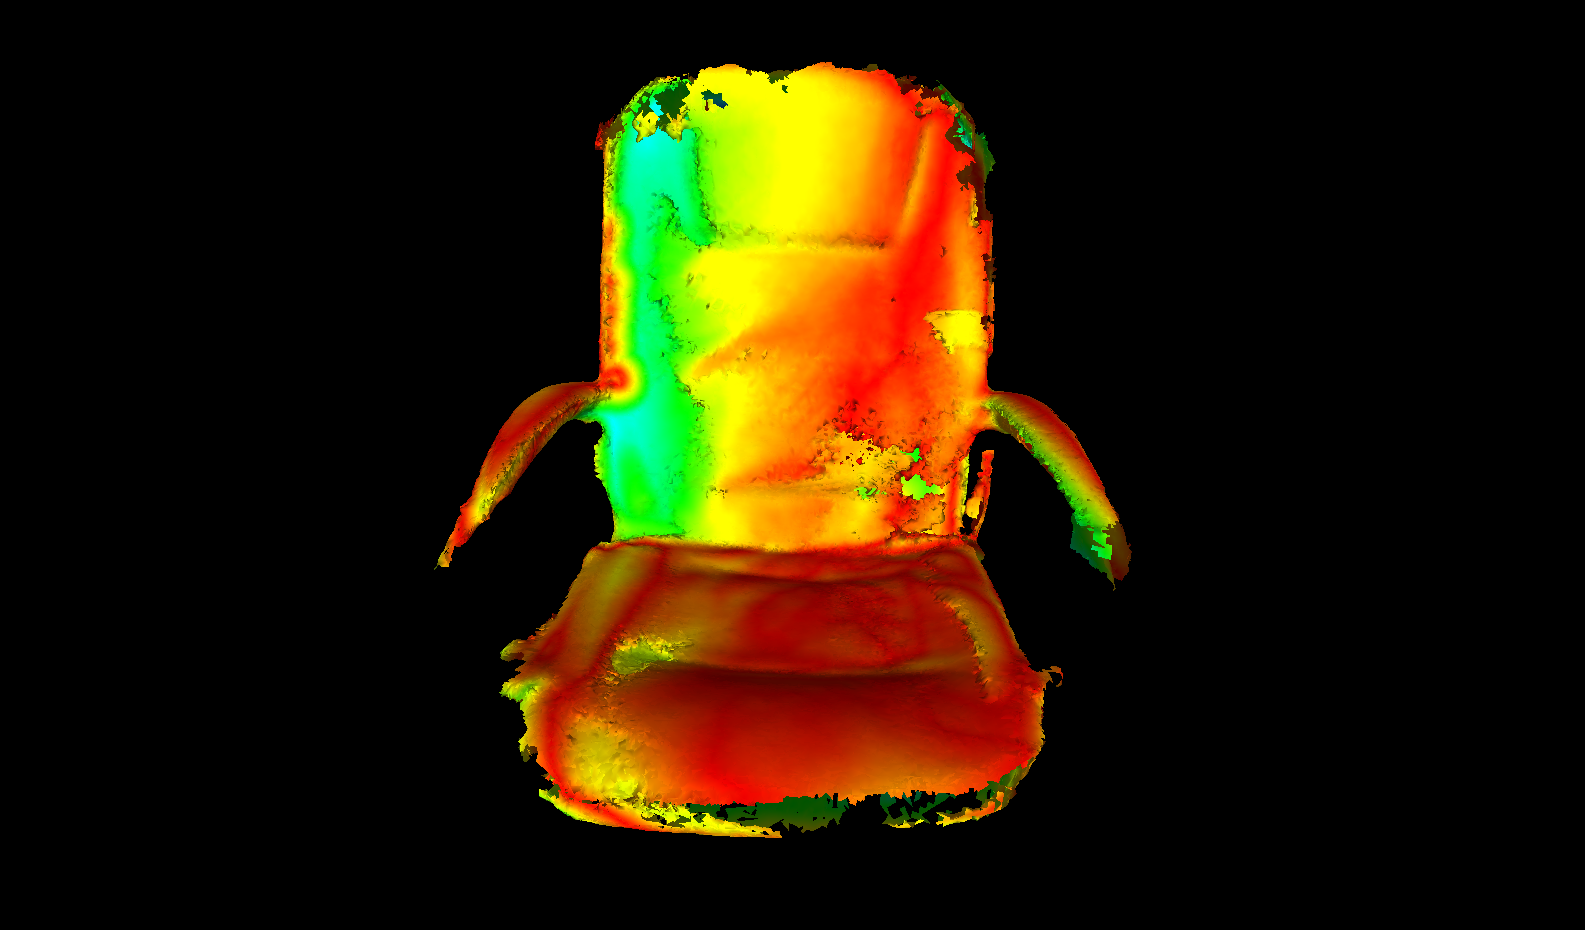
\includegraphics[width=3cm]{hausdorff/chair.png}}&
		\fbox{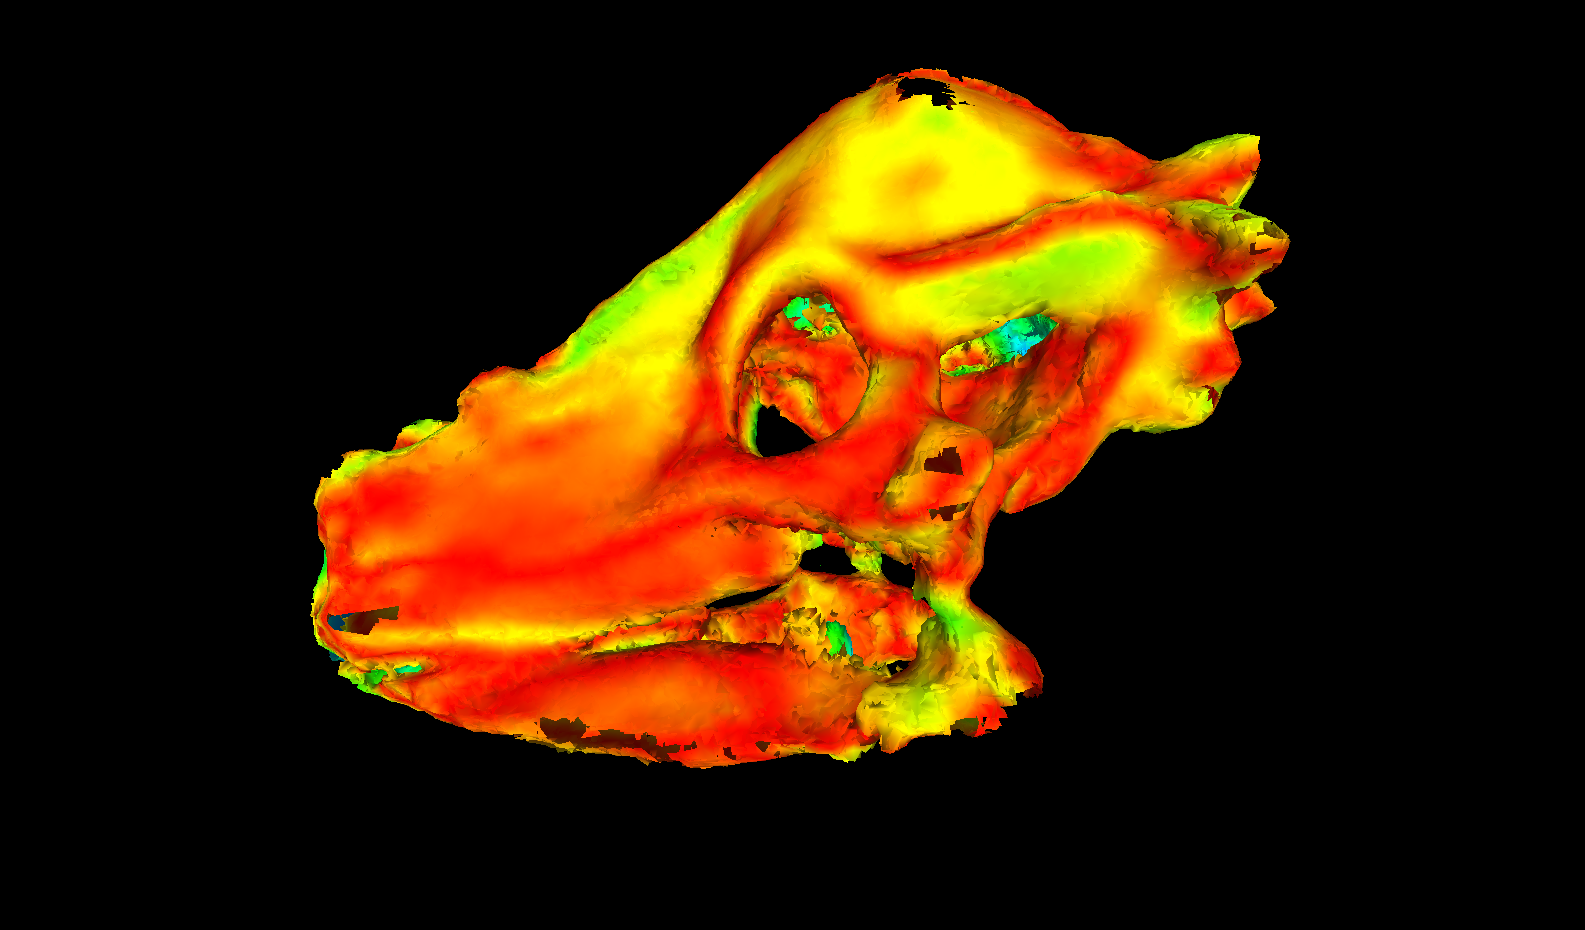
\includegraphics[width=3cm]{hausdorff/dino.png}}\\
		(a)&(b)&(c)&(d)
	\end{tabular}
	\vspace{1mm}
	
	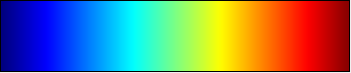
\includegraphics[scale=0.5]{hausdorff/colour_range.png}\\
	(e)
	
	\caption{
		Reconstructions textured by Hausdorff Distance to ground truth:
		\textbf{(a)} Bear,
		\textbf{(b)} Brain,
		\textbf{(c)} Chair,
		\textbf{(d)} Dino,
		\textbf{(e)} Relative distance scale.
	}
	%	\vspace{-5mm}
	\label{fig:hausdorffTextured}
\end{figure*}

As can be seen by the similarity measures presented, our system is capable of yielding reconstructions to a high quality despite the much more difficult tracking scenario of a single object rather than an entire 
scene. It can be seen that our output reconstruction meshes are geometrically close to those generated with a dense SLAM system \cite{Prisacariu2014} following the KinectFusion \cite{Newcombe2011} pipeline that 
is modelling and tracking the entire scene.

\subsection{Running Times and Performance}
We have implemented our system both on the CPU and GPU. With a GPU implementation with NVIDIA CUDA we are able to achieve runtimes of on average \textit{90Hz} with a consumer grade NVIDIA GeForce GTX1060 with 
6GB GRAM. With our CPU only implementation we make use of parallelism with OpenMP and achieve runtimes of on average \textit{5Hz} on a consumer grade PC with an Intel Core i5-6600K 3.5GHz CPU and 16GB of RAM. Such 
online runtimes are possible due to the asynchronous way in which we have implemented the online adjustments combined with GPU acceleration